\chapter{Software operations}
\label{chap:soptware_operations}


\section{Create a new crisis event}
\label{operation:MyOperation}
The central coordinator creates and adds a new crisis event to the system after
being informed by a third party (citizen, organization).

\begin{description}

\item \textbf{Parameters:} Information of Witness, Crisis Information, Fireman
Coordinator.
\item \textbf{Precondition:} The central coordinator is logged in and has
received information from a witness.
\item \textbf{Post-condition:} A new crisis has been added to the system and the
new crisis has automatically been assigned to a fireman coordinator, who has
received an automatic notification from the system.
\item \textbf{Output messages:}\begin{enumerate}\item The selected fireman
coordinator will be notified automatically once the crisis has been created.
\item A new crisis with the corresponding information will be added to the
central coordinator's graphical user interface.
\end{enumerate}

\item \textbf{Triggering:}
\begin{enumerate}
\item From within the crisis management window fill out the required entries
related to the personal information of the witness such as name and actor type.
\item Fill out the comment entry related to the crisis.
\item Click the “Get Location” button.
\item Click on the “Confirm Location” button, then click on the “Submit”
button and add the entry to the database.
\end{enumerate}

 
\end{description}

 
\subsection{Create a new crisis event example}
To create a new crisis event, the central coordinator clicks on the “Add Event”
button (see Fig. 4.1). A new window appears, where the central coordinator fills
in all the provided information of the witness (see Fig. 3.1). Then the central
coordinator clicks on the “Get Location” button to tell the system to get the gps coordinates of the phone
number of the witness (see Fig. 3.1). Then, after oraly checking with the
witness that the gps coordinates are correct, the central coordinator clicks on
the “Confirm Location” button.
Finally the central coordinator can submit the new crisis event and add it to
the database by clicking on the “Submit” button. After the successfull creation
of a new crisis event, the event is shown in the graphical user interface of the
central coordinator (see Fig. 4.2) and the nearest fireman coordinator to the
gps coordinates is notified.
\begin{minipage}{1.0\textwidth}
\begin{figure}[H]
\caption{New event button}
\includegraphics[width=0.9\textwidth]{Add_event.eps}
\end{figure}
\end{minipage}

\begin{minipage}{1.0\textwidth}
\begin{figure}[H]
\caption{Active events in GUI}
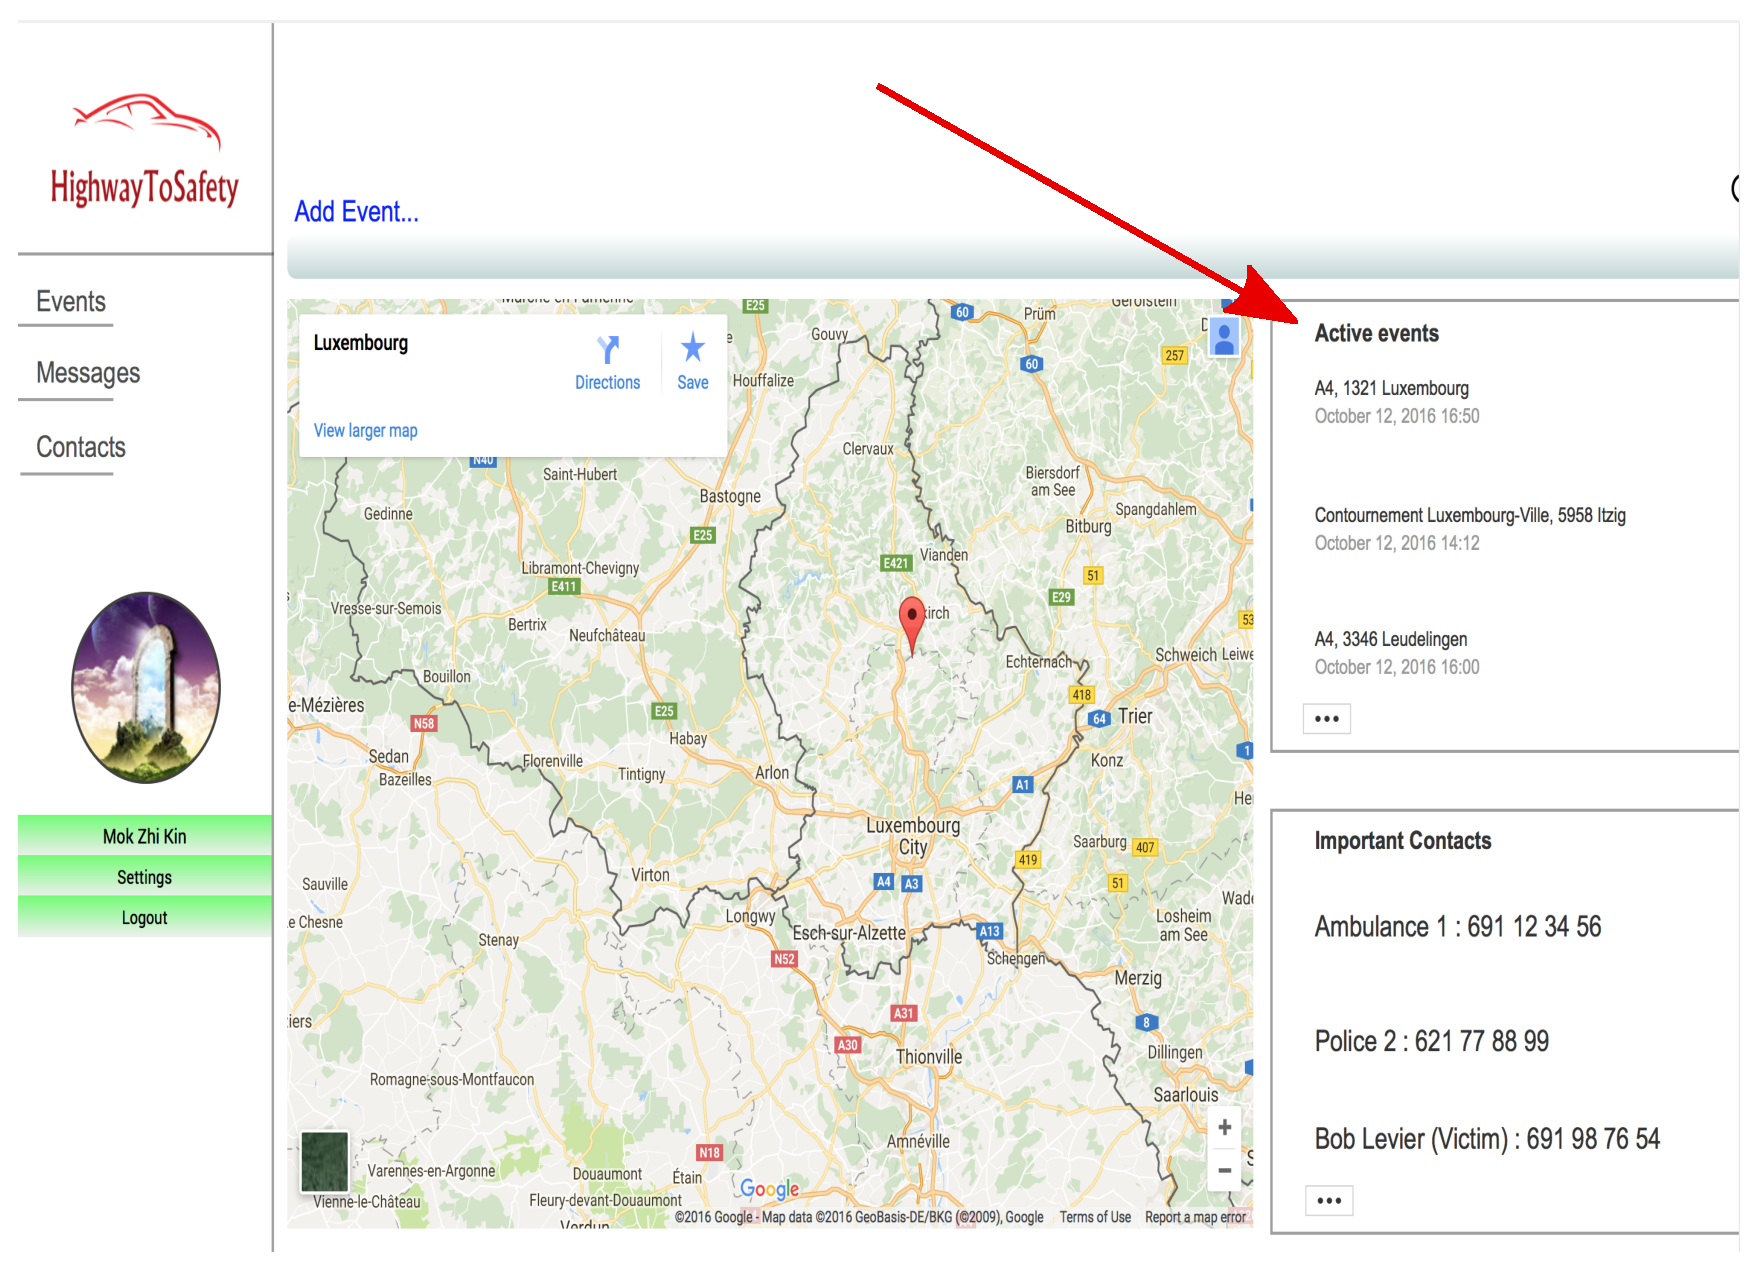
\includegraphics[width=0.9\textwidth]{Active_events.eps}
\end{figure}
\end{minipage}



\section{Send a message to the Emergency Central}
\label{operation:MyOperation}
The fireman coordinator writes a message and then sends it to the central
coordinator, either by typing in text or by using the preprogrammed macros.

\begin{description}

\item \textbf{Parameters:} Typed-in text, Quantity of assistance.
\item \textbf{Precondition:} The fireman coordinator is logged into the Ipad
app.
\item \textbf{Post-condition:} A new message has been send to the central
coordinator. 
\item \textbf{Output messages:}
\begin{enumerate}
  \item The fireman coordinator sees in the chat log that the message went out.
  \item The message displays in the GUI of the central coordinator.
\end{enumerate}

\item \textbf{Triggering:}
\begin{enumerate}
  \item From the main menu of the Ipad App click on the “Chat” button.
  \item In the chat window, you can choose rather to use the preprogrammed
  macros or to type in text manually.
  \item To use the macros you have to choose what kind of assistance you need
  (Ambulance, Police, Firetruck) and select the quantity you need, then you
  press the button with the wished assistance.
  \item To write customized messages, you can use the input field which says
  “write here\ldots”.
\end{enumerate}
\end{description}

 
\subsection{Send a message to the Emergency Central example}
The fireman coordinator wants to send a message to inform the central
coordinator that they need 3 more policemen. The fireman coordinator clicks on
the “Chat” button to enter the chat window (see Fig. 4.3). The fireman
coordinator sets the value next to the police logo to 3 and clicks on the
police logo(see Fig.4.4).
After the successfull sending of the message, the message
appears in the chat log of the fireman coordinator and on the GUI of the central
coordinator under the “Messages” window (see Fig.4.4).

\begin{minipage}{1.0\textwidth}
\begin{figure}[H]
\caption{Main menu of Ipad app}
\includegraphics[width=0.9\textwidth]{IpadAppHome1.eps}
\end{figure}
\end{minipage}

\begin{minipage}{1.0\textwidth}
\begin{figure}[H]
\caption{Chat menu of Ipad app}
\includegraphics[width=0.9\textwidth]{Chat_Example.eps}
\end{figure}
\end{minipage}

\section{Update Status on Ipad Application}
\label{operation:MyOperation}
The coordinator, who uses the Ipad, updates his status to inform the system if
his team is stil in “Staion”, “In transit” or already “Arrived”

\begin{description}

\item \textbf{Parameters:} Status input.
\item \textbf{Precondition:} The coordinator's Team is in a certain status and
the coordinator is logged into the Ipad app.
\item \textbf{Post-condition:} The coordinator's Team is in another status then
in the Precondition.
\item \textbf{Output messages:} The central coordinator of the emergency central
receives a message that the status of the coordinator's team has been updated in
the system and the changes are displayed in his GUI.

\item \textbf{Triggering:} 
\begin{enumerate}
  \item From the main menu of the Ipad App click on the “Map” button.
  \item In the map window click on the menu underneath the “Status:” label and
  select the status you want to update to.
\end{enumerate}
\end{description}

 
\subsection{Update Status on Ipad Application example}
In the main menu of the Ipad app, the coordinator of a team clicks on the “Map”
button to open the map window (see Fig. 4.3). In the map window the user clicks
on the menu underneath the “Status:” label and selects the status “Arrived” to tell the system that the
team has arrived on the accidesnt's location (see Fig. 3.2).

\section{Update Map on Ipad Application}
\label{operation:MyOperation}
The coordinator, who uses the Ipad, updates the map to get the newest
information on his map, like traffic information, accident location information or location
of other parties like ambulance, tow-truck, police.

\begin{description}

\item \textbf{Parameters:} 
\item \textbf{Precondition:} The Ipad user is on the “Map” window of
the Ipad app.
\item \textbf{Post-condition:} The map is updated and shows all the new
information.
\item \textbf{Output messages:} The map of the “Map” window changes.


\item \textbf{Triggering:}
\begin{enumerate}
  \item From the main menu of the Ipad App click on the “Map” button.
  \item Click on the “Update” button.
\end{enumerate}
 

\end{description}

 
\subsection{Update Map on Ipad Application example}
In the main menu of the Ipad app, the user clicks on the “Map” button to open
the map window (see Fig. 4.3). In the map window the user clicks on the “Update”
button to update the map. After a few seconds the updated map is displayed and all the
newest information is shown.
